% PLEASE USE THIS FILE AS A TEMPLATE
% Check file iosart2c.tex for more examples
%
% Journal:
%   Journal of Ambient Intelligence and Smart Environments (jaise)
%   Web Intelligence and Agent Systems: An International Journal (wias)
%   Semantic Web: Interoperability, Usability, Applicability (SW)
% IOS Press
% Latex 2e

% options: jaise|wias|sw
% add. options: [seceqn,secfloat,secthm,crcready,onecolumn]


\documentclass{iosart2c}

%\documentclass[sw]{iosart2c}
%\documentclass[wias]{iosart2c}
%\documentclass[jaise]{iosart2c}

\usepackage[T1]{fontenc}
\usepackage{times}%
\usepackage{natbib}% for bibliography sorting/compressing
%\usepackage{amsmath}
%\usepackage{endnotes}
\usepackage{graphicx}

%%%%%%%%%%% Put your definitions here
\usepackage[utf8]{inputenc}
\usepackage[hyphens]{url}
\usepackage{verbatim} 
\usepackage[pdftex,urlcolor=black,colorlinks=true,linkcolor=black,citecolor=black]{hyperref}
\def\sectionautorefname{Section}
\def\subsectionautorefname{Subsection}
% bullet numbers
\usepackage{tkz-graph}
\usetikzlibrary{matrix,arrows,decorations.pathmorphing,shapes}
\newcommand{\dobulletnumber}[1]{\node[circle,text=white,fill=gray,anchor=west,inner sep=1pt] {\sffamily #1}}
\newcommand{\bulletnumber}[1]{\tikz[baseline=-2.5,overlay]\dobulletnumber{#1};}
\newcommand{\bulletref}[1]{\tikz[baseline=-2.5]\dobulletnumber{\fontsize{8}{8}\selectfont#1};}
% todo macro
\usepackage{color}
\newcommand{\todo}[1]{\noindent\textcolor{red}{{\bf \{TODO}: #1{\bf \}}}}

%% Define a new 'smallurl' style for the package that will use a smaller font.
\makeatletter
\def\url@smallurlstyle{%
  \@ifundefined{selectfont}{\def\UrlFont{\sf}}{\def\UrlFont{\scriptsize\ttfamily}}}
\makeatother
%% Now actually use the newly defined style.
\urlstyle{smallurl}
\newcommand{\nofootnote}[1]{~#1}

%%%%%%%%%%% End of definitions

\pubyear{0000}
\volume{0}
\firstpage{1}
\lastpage{1}

\begin{document}

\begin{frontmatter}

\pretitle{What'chu talkin' about, Willis?}
\title{A Comparison of Topics People read about on Facebook and on Twitter and where}
%\subtitle{}

%\footnote{\url{http://en.wikipedia.org/wiki/Diff'rent\_Strokes\#Later\_appearances\_of\_the\_characters}}

\runningtitle{A Comparison of Topics People read about on Facebook and on Twitter and where}

%\review{}{}{}

% Two or more authors:
\author[A]{\fnms{Thomas} \snm{Steiner}\thanks{T. Steiner is partially supported by the European Commission under Grant No. 248296 FP7 I-SEARCH project}},
\author[B]{\fnms{Arnaud} \snm{Brousseau}\thanks{A. Brousseau was an intern at Google Germany GmbH at the time of writing.}},
\author[C]{\fnms{Raphaël} \snm{Troncy}},
\author[D]{\fnms{Ruben} \snm{Verborgh}},
\author[E]{\fnms{Rik} \snm{Van de Walle}},
\author[F]{\fnms{Joaquim} \snm{Gabarró Vallés}}

\runningauthor{T. Steiner, A. Brousseau, R. Troncy, R. Verborgh, et al.}

\address[A]{Google Germany GmbH, ABC-Str. 19, 20354 Hamburg, Germany,\\
E-mail: tomac@google.com}
\address[B]{Google Germany GmbH, ABC-Str. 19, 20354 Hamburg, Germany,\\ 
E-mail: arnaud.brousseau@gmail.com}
\address[C]{EURECOM, Sophia Antipolis, France\\
E-mail: raphael.troncy@eurecom.fr}
\address[D]{Ghent University -- IBBT, ELIS, Multimedia Lab, Gaston Crommenlaan 8/201, 9050 Ghent, Belgium,\\
E-mail: ruben.verborgh@ugent.be}
\address[E]{Ghent University -- IBBT, ELIS, Multimedia Lab, Gaston Crommenlaan 8/201, 9050 Ghent, Belgium,\\
E-mail: rik.vandewalle@ugent.be}
\address[F]{Universitat Polit\`{e}cnica de Catalunya, Department LSI, 08034 Barcelona, Spain,\\
E-mail: gabarro@lsi.upc.edu}

\begin{abstract}
\todo{Write abstract}
\end{abstract}

\begin{keyword}
\todo{List keywords}
\end{keyword}

\end{frontmatter}

%%%%%%%%%%% The article body starts:

\section{Introduction} \label{sec:introduction}
In recent years, social media mining has become an essential tool for marketers, traders, and researchers.
The information people share publicly on social networks harbors tremendous amounts of valuable social data.
Forbes have called the social graph \emph{crude oil} in a recent blog post~\cite{ForbesPost}.
Social networks today are very much ``walled gardens'', excellently illustrated by a cartoon by David Simonds~(\autoref{fig:DavidSimonds}).
This network isolatedness reflects on how social media mining is done nowadays.
Common literature typically either focuses on just one network~\cite{russell201121}, or treats the different networks separately~\cite{russell2011mining}.
Social media mining happens based on either keyword-based search APIs, or so-called ``fire hose'' realtime streaming APIs, both provided by the social networks themselves.
The main difference is that in the prior case terms like the name of a brand or company are \emph{proactively} searched for, whereas in the latter case the social media mining system \emph{reactively} acts upon the occurrence of such terms.

In this paper, we consider the two popular social networks Facebook\footnote{\url{http://facebook.com/}} and Twitter\footnote{\url{http://twitter.com/}}.
Traditionally, Twitter is very open with their API, as since the beginning of the platform, API-based Twitter clients have played a strategic role for the company.
Twitter provides developers with the Twitter Streaming API~\cite{TwitterStreamingAPI}, which allows high-throughput near-realtime access to various subsets of public and protected Twitter data.
Facebook has no such public ``fire hose'' API, however, via its Graph API~\cite{FacebookRealtimeAPI} supports realtime updates to enable applications to subscribe to a limited set of changes in data from Facebook.
Whenever a subscribed change occurs, Facebook notifies subscribers with a list of changes.
This imbalance of API openness has an impact on publications around social networks.
While at the \textit{World Wide Web Conference 2011} alone three Twitter papers based on the Twitter API were published~\cite{Romero:2011:DMI:1963405.1963503, Meeder:2011:WKY:1963405.1963479, Wu:2011:SWT:1963405.1963504}, publications on Facebook typically focus on privacy issues~(e.g.,~\cite{liu:settings}), or Facebook's sociological impact~(e.g.,~\cite{JCC4:JCC4367}), without making use of the Facebook API.

What to the best of our knowledge all publications so far have in common is their focus on the author side, i.e., it is very well researched what people \emph{produce} on social networks -- and especially on Twitter -- however, not so much what people \emph{consume}.
This is especially true across social networks.
As far as we can tell, no study has compared \emph{reader} behavior on different social networks before.
In this work, we compare topics people read about on Facebook and on Twitter and classify those topics in order to provide an overall comparison.
We therefore have implemented two similar browser extensions, one for Twitter, one for Facebook, that enrich the user experience on those social networks and by means of a named entity disambiguation tool determine the topics that people see on their timelines.
By focusing exclusively on content people see when navigating to either \url{http://twitter.com} or \url{http://facebook.com}, we assume people indeed read that content, especially as both social network sites require users to actively click a link ``$\mathit{n}$ new stories since your last visit'' or ``$\mathit{n}$ new tweets'' respectively rather than auto-updating the timeline.

\subsection{Paper Objective and Structure}
In this paper, we \textbf{will not}:
\begin{itemize}%[topsep=-.5em, partopsep=0pt, itemsep=0pt]
	\item perform analyses based on hashtags, term frequency, or trends;
	\item perform analyses based on geotagged microposts;
	\item work with huge amounts of microposts from ``fire hose'' APIs;
	\item focus on the micropost author side.
\end{itemize}
On the contrary, we \textbf{will}:
\begin{itemize}%[topsep=-.5em, partopsep=0pt, itemsep=0pt]
	\item perform analyses based on disambiguated named entities;
	\item perform analyses based on IP-based reader location detection;
	\item work with a manageable amount of microposts read by a random population of social network users;
	\item focus on the micropost reader side,
\end{itemize}
which is why we strive for a paradigm shift that promises new insights for tasks like brand analysis, opinion research.

\todo{Describe paper structure.}


\begin{figure}
\centering
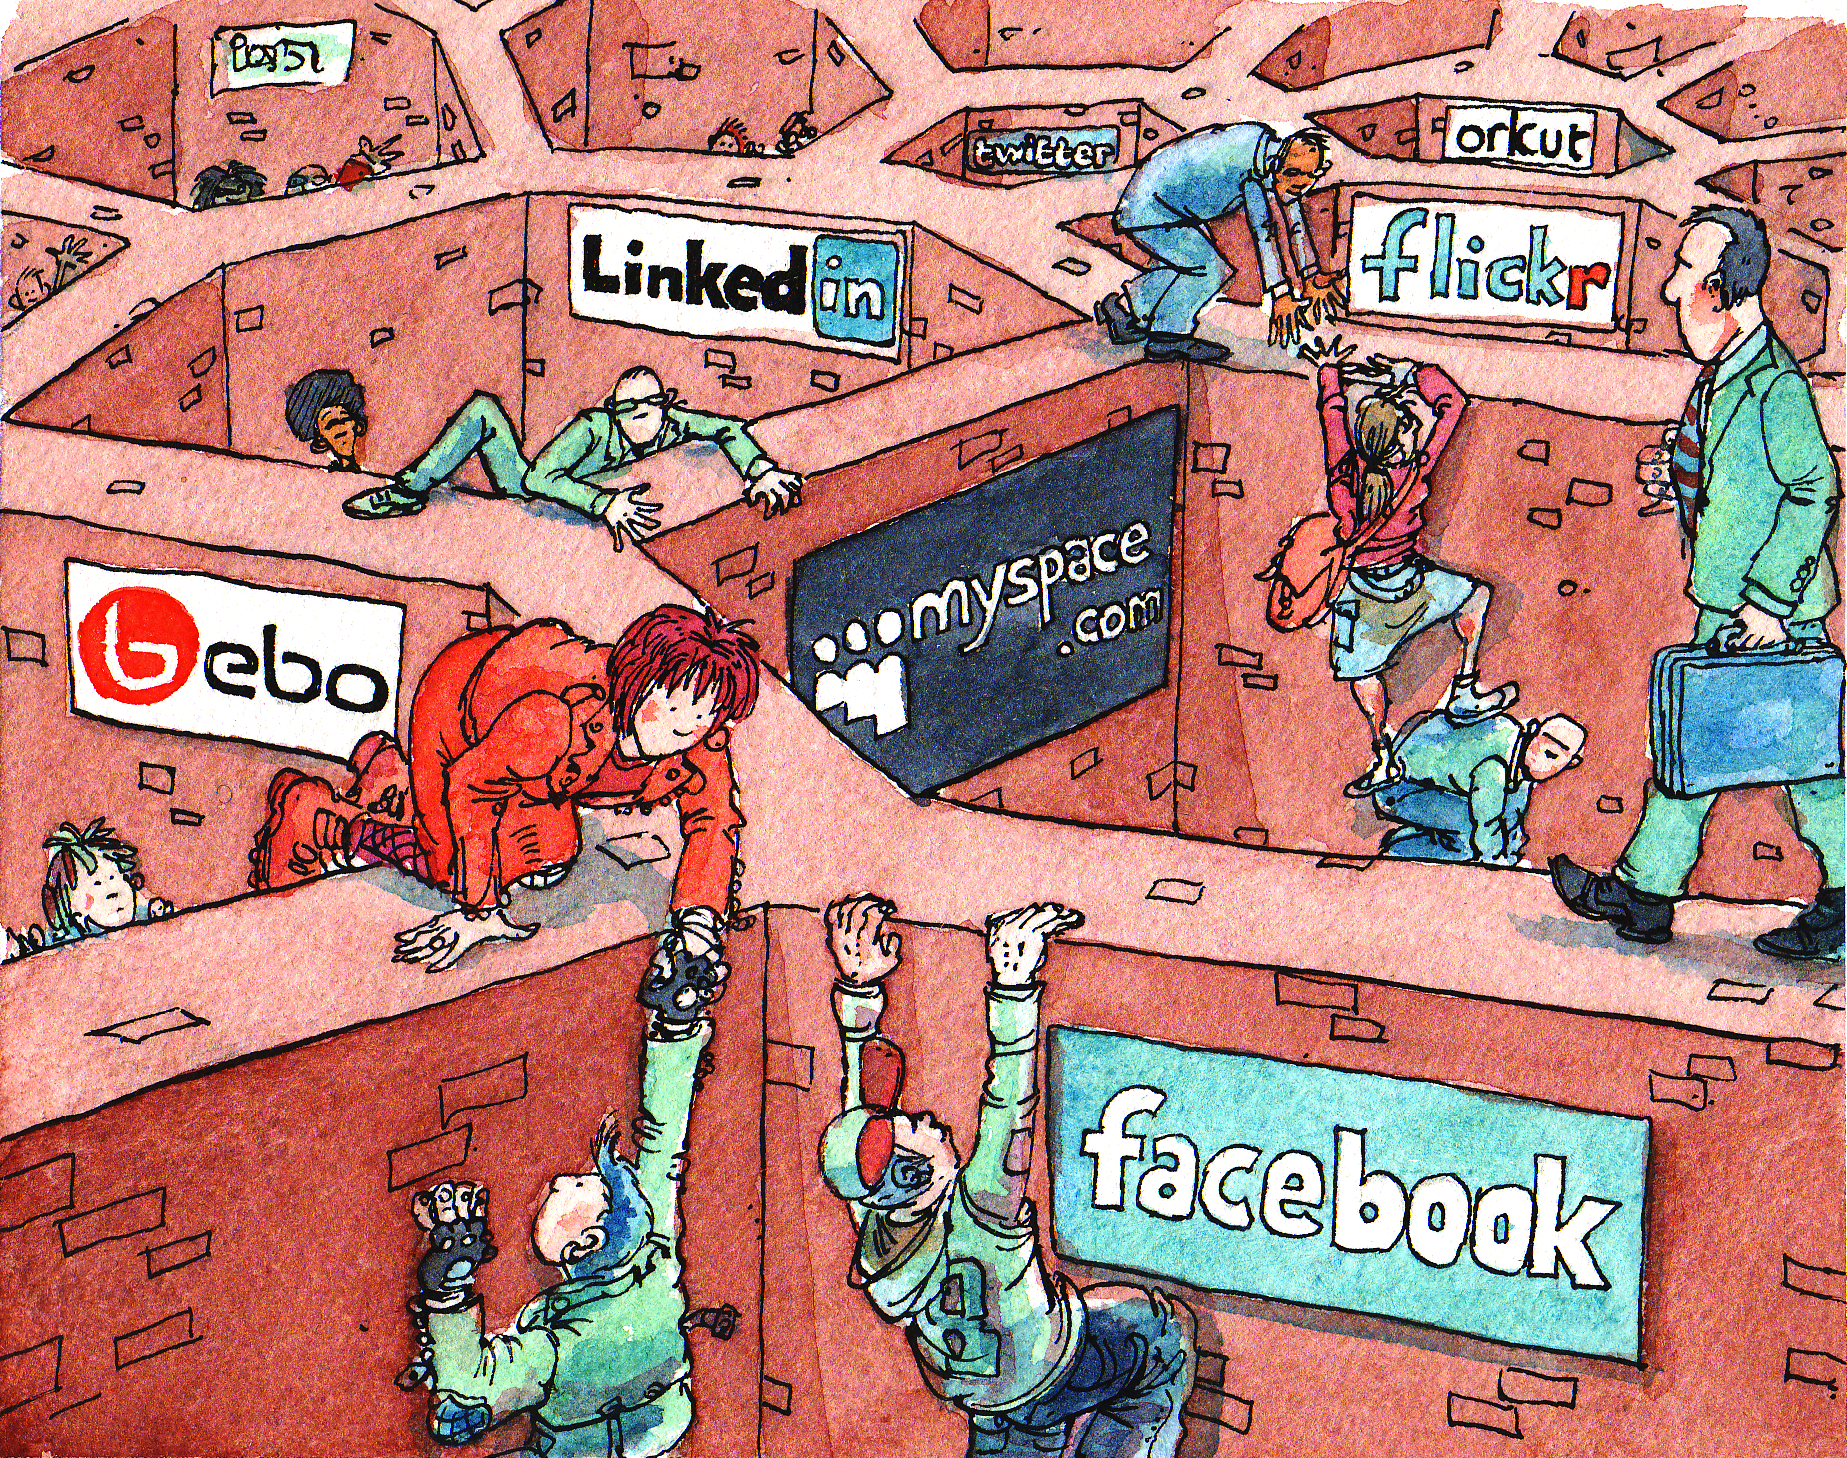
\includegraphics[width=1.0\linewidth]{./resources/davidsimonds.png}
\caption{Social networks as walled gardens.~\cite{DavidSimonds}}
\label{fig:DavidSimonds}
\end{figure}

\section{Implementation} \label{sec:implementation}

\begin{figure}
\centering
\includegraphics[width=1.0\linewidth]{./resources/twitterswarmnlpstats.png}
\caption{\textit{Seven day active users} development for the Twitter Swarm NLP browser extension.}
\label{fig:twitterswarmnlpstats}
\end{figure}

\begin{figure}
\centering
\includegraphics[width=1.0\linewidth]{./resources/facebookswarmnlpstats.png}
\caption{\textit{Seven day active users} development for the Facebook Swarm NLP browser extension.}
\label{fig:facebookswarmnlpstats}
\end{figure}

\section{User Demographics} \label{sec:userdemographics}
We have released the two browser extensions independent of each other on the Chrome Web Store\footnote{https://chrome.google.com/webstore/category/home}. The extension descriptions contain full disclosure on the collected data and on the usage of a Web analytics tool. As the extensions inject the Google Analytics tracking snippet, exact user localization is possible based on the users' current physical location, i.e., completely independent from the origin location users might have registered with Twitter or Facebook. A graphical overview of user locations can be seen in~\autoref{fig:twitterlocation} and~\autoref{fig:facebooklocation}. The complete statistics can be found online\footnote{\todo{Provide URL of full statistics}}.

In the period from March 1 to November 8, for Facebook Swarm NLP, overall 858 unique Facebook users accessed the extension at least 10 times, in comparison to overall 86 unique Twitter Swarm NLP users. If we put these figures in contrast with the \emph{seven day active users} statistics for the extensions (~\autoref{fig:facebookswarmnlpstats} and \autoref{fig:twitterswarmnlpstats}), where Facebook reached 135 and Twitter Swarm NLP 72 seven day active users as of November 6, we can derive that Twitter users mostly installed the extension and stayed with it, whereas Facebook users installed the extension, used it for a while, and uninstalled it.

\begin{figure}
\centering
\includegraphics[width=1.0\linewidth]{./resources/twitterlocation.png}
\caption{Location of users of the Twitter Swarm NLP browser extension (Mar. 1 -- Nov. 8).}
\label{fig:twitterlocation}
\end{figure}

\begin{figure}
\centering
\includegraphics[width=1.0\linewidth]{./resources/facebooklocation.png}
\caption{Location of users of the Facebook Swarm NLP browser extension (Mar. 1 -- Nov. 8).}
\label{fig:facebooklocation}
\end{figure}

\section{Discussion}
% Talk about what network to use for what purpose, talk about brand analysis etc.

\section{Related Work} \label{sec:relatedwork}

\section{Future Work and Conclusion} \label{sec:futureworkandconclusion}

%%%%%%%%%%% The bibliography starts:
\bibliographystyle{abbrv}
\bibliography{swj2012}

\end{document}